This section describes the mechanisms implemented in the Lightning network to support payments.

We model the Lightning network as a undirected graph $\langle N,C \rangle$, being N the Lightning \textit{nodes} and $C$ the \textit{channels}, that allow payments between two nodes.
Although the funding supporting a lightning channel is provisioned by one of the two nodes it connects,
it allows transactions started by any of them provided that the node initiating the transaction has enough positive balance. 
Therefore, Lightning channels are deemed to be \textit{bidirectional}.
We denote the channels as $C_{i,j}$, to represent a channel between $N_i$ and $N_j$, 
starting for convenience with the node that provisioned the funds (i.e., $N_{i}$ for $C_{i,j}$). 
As many channels can be set between the same pair of nodes, we denote them as $C'_{i,j}$, $C''_{i,j}$, etc.
Figure~\ref{fig:lightning-topology} shows an example of a Lightning topology.
% There can be more than 1 channel between two nodes
We define the capacity of channel $C_{i,j}$ from $N_i$ to $N_j$, denoted $\lambda_{i,j}$, 
%($\lambda'_{i,j}$, etc.), 
the amount of currency that can be transferred from $N_i$ to $N_j$ at the current moment. 
Then, with $\Lambda_{i,j}$ we denote the initial amount of currency funded by node $N_i$,
\begin{equation}
    \lambda_{j,i} = \Lambda_{i,j} - \lambda_{i,j}
\end{equation}

\begin{figure}[h!]
    \centering
    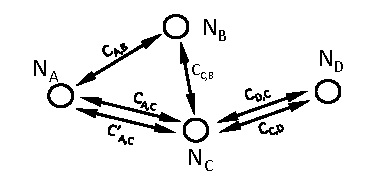
\includegraphics[width=0.95\linewidth]{img/lightning-topology.pdf}
    \caption{Example of Lightning topology}
    \label{fig:lightning-topology}
\end{figure}

The Lightning network~\cite{poon2016bitcoin} allows payments between nodes $N_i$ and $N_k$ that are not directly connected through a channel,
by means of relying in a sequence of nodes that act as intermediary parties.
The first node in the path must transfer the desired amount (plus appropriate fees) to the second, this to the third, and so on, until the destination receives the payment. 
Consensus on the completion of this operation is achieved by a sequence of pair-wise agreements, 
called bilateral \textit{hash time locked contracts}~\cite{BOLT_5_transaction_handling},
that guarantee that either every node involved receives the corresponding amount, or no one does.
These agreements are carried off-chain, in the sense that do not need to be registered in the blockchain to be trusted, 
although they can be when a channel is closed. 
%The mechanism ensures that either all the nodes receive the prove of the transaction, or neither of them can claim that …


To issue a transaction, the sender defines the intermediate channels through which the transaction will proceed. 
This path must be complete, in the sense that every channel traversed must be specified in advance.
Such a forwarding mechanism is usually known as \textit{strict source routing}~\cite{BOLT_4_onion_routing}.
To be able to discover channels, and thus build paths, nodes connect to other nodes already part of the network and exchange routing information. 
When a node connects first to a node part of the Lightning network, it receives the list of nodes and channels known by its peer~\cite{BOLT_7_routing_gossip}. 
Channel information includes source and destination channel endpoints (e.g., $i$ and $j$, respectively) 
and policy information referred to the channels: the funding capacity $\Lambda_{i,j}$ for the channel, the fee required for performing a payment, or the time lock during which the transaction [???]. 
The advertised capacity value for a channel $C_{i,j}$ corresponds to the value $\Lambda_{i,j}$ committed in the funding transaction creating the channel. 
Besides this initial information, nodes receive and propagate updates such as new channels added or channels closed.

When two nodes $N_i$ and $N_j$ have established a Lightning connection, they can negotiate the set up a new channel. 
In this negotiation, they build a multisignature Bitcoin address, so that the associated funds can only be retrieved under the agreement of both parties~\cite{poon2016bitcoin}.
Then, one of the nodes, e.g., $N_i$, performs a transaction in the Bitcoin blockchain, the funding transaction, to the multisignature address. 
The value of this transaction is the maximum amount of currency that can be transferred from $N_i$ to $N_j$.
The channel can now be advertised to other nodes, with the capacity set in the funding transaction, and the fees that they will apply to payments over the channel, that they exchanged in the channel setup negotiation.

Once created the channel, $N_i$ (and later $N_j$, when it has positive balance) can start issuing payments. 
These payments are executed as contracts they sign to each other, which are tied to time conditions (time-locks), in a way that any of the parties can eventually write the contract as a blockchain transaction that is executed to distribute the funds according to the last agreement and close the channel~\cite{BOLT_5_transaction_handling}. 
However, the channel does not need to be closed after a single transaction, but the contracts exchanged off-line (without blockchain registry) can keep an updated view of the balance of the parties over time.

Nodes willing to initiate a payment to a destination not directly connected through 
a channel use the routing information they have to compute 
paths with enough declared capacity to complete the transaction. 
Note that the current capacity can be different than this, as previous transactions may have altered the balance, 
and these changes are not advertised through the routing system.
Once defined the path by the initiator, a payment request 
is forwarded through it. 
When a node in the path receives the request, it checks if the next node is active - e.g., the node may be temporarily offline.
Then, the node checks if
actual channel capacity for the egressing channel suffices for the payment. 
If any of the checks fail, it reports an error to the source node, indicating the node that detected it, and the operation is aborted.
However, in case of low capacity, the node does not indicate the available capacity.

If all the nodes are connected, and have enough capacity, so the request arrives to the destination, then
the pair-wise hash time-locked contract machinery starts its operation~\cite{BOLT_2_channel_management, BOLT_5_transaction_handling}.


